\chapter{L’exemple des myopathies congénitales et la difficulté du diagnostic}
notre cas d'application on va parler des myopathies et voir comment on peut utiliser l'IA pour analyser les données
Avec une attention particulière aux myopathies congénitales, leur classification et leur diagnostic.

\section{Le muscle, un organe avec une structure cellulaire particulière}
nombre de muscle, fonction, pourcentatages
Différrents types de muscles 

\subsection{Type de Muscle}
Muscle cardiaque

Muscle lisse

Muscle striée
\begin{figure}[!htbp]
 \centering
 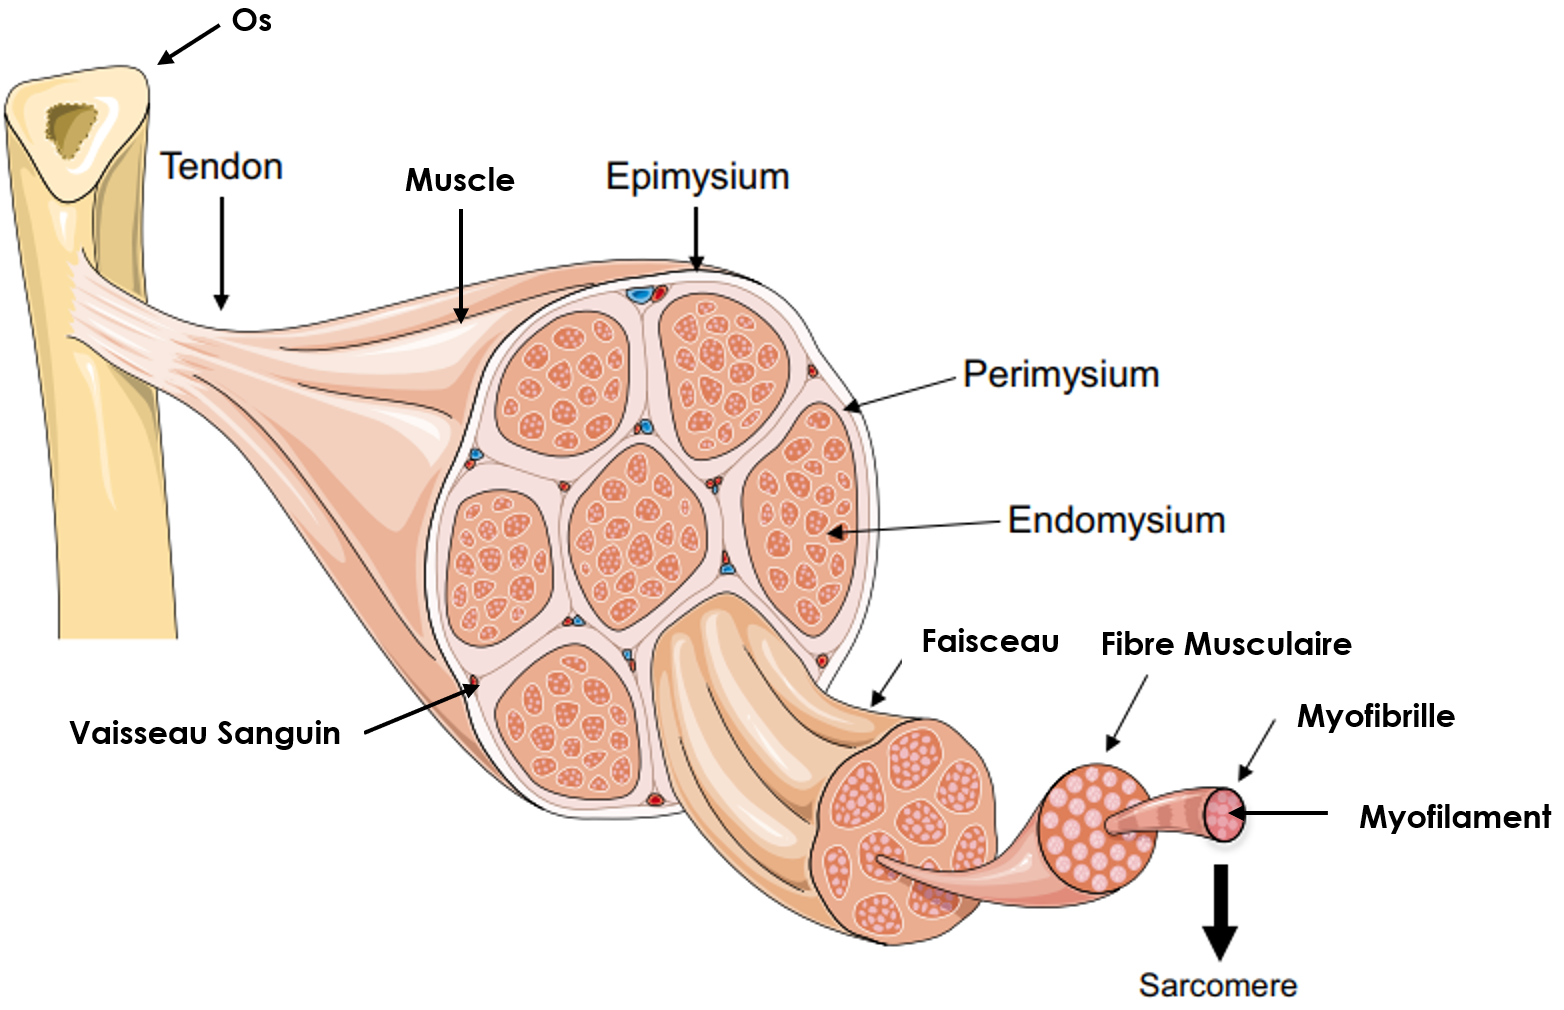
\includegraphics[width=0.8\textwidth]{figures/muscle.png}
 \caption[Schéma de l'architecture du modèle enformer]{Schéma de l'architecture du modèle enformer. Ce modèle basé sur les \textit{transformers} permet de prendre jusqu'à 100 000 paires de bases de contexte génomique pour évaluer l'expression d'un gène (\cite{avsec_effective_2021}).}
 \label{fig:enformer}
\end{figure}

\begin{figure}[!htbp]
 \centering
 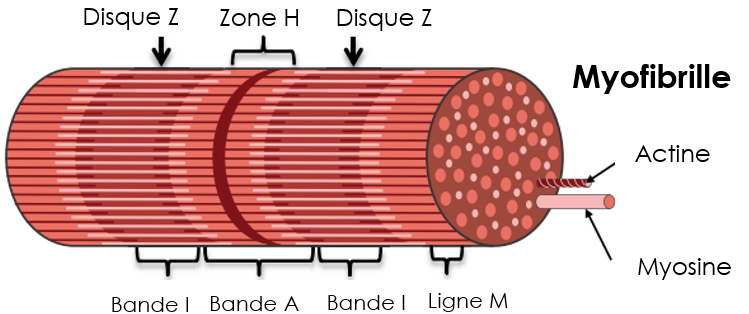
\includegraphics[width=0.8\textwidth]{figures/sarcomere.png}
 \caption[Schéma de l'architecture du modèle enformer]{Schéma de l'architecture du modèle enformer. Ce modèle basé sur les \textit{transformers} permet de prendre jusqu'à 100 000 paires de bases de contexte génomique pour évaluer l'expression d'un gène (\cite{avsec_effective_2021}).}
 \label{fig:enformer}
\end{figure}


\subsection{Strucutre}

fibre musculaire entourée d'une membrane: le sarcolemme

\subsection{Type de fibres musculaires, fonctionnement}
tableau des caractéristiques fibre 1 2A 2B

\subsection{Atteinte neuromusculaires}
tableau des NMD

\section{Les myopathies congénitales}

\subsection{Description générale}
les types
traitement ?

\subsection{Prévalence}
\subsection{Classification}


\section{Données générées pour le diagnostic des myopathies congénitales}
\subsection{Diagnostic}
les colorations de routines

L’Atlas du Muscle : une banque d’images
de biopsies musculaires
Norma B. Romero, Bruno Cadot
